\chapter{Technology Review}
This chapter discusses the different technologies used in throughout the project. It discusses the the advantages and disadvantages of each technology and why certain technologies were used over others.

\section{Overview}
This project is comprised of React as the frontend, Flask as the server which is hosted on PythonAnywhere, MongoDB as the database, and ... to host the application. Throughout the project, the following technologies were also used and tested before the above was ultimately chosen:
\begin{itemize}
    \item Angular/Ionic
    \item Firebase
    \item Django
    \item MySQL
    \item Amazon Web Services
\end{itemize}

\section{Main Technologies}
This section will discuss the main technologies currently in use in the web application. The preceding section will discuss other technologies tried but ultimately weren't incorporated. 

\newpage

\subsection{React}
\par
\medskip
\begin{center}
    
\includegraphics[width=8cm,height=3.3cm,keepaspectratio]{images/react}
\end{center}
React (also known as React.js or ReactJS) is a JavaScript library for building user interfaces. It is maintained by Facebook and a community of individual developers and companies.

React can be used as a base in the development of single-page or mobile applications. However React is only concerned with rendering data to the DOM and so creating React applications usually requires the use of additional libraries for state management and routing. Redux and React Router are respective examples of such libraries. 

\subsubsection{Advantages}
React has many advantages, several of which apply to this project:

% https://www.altexsoft.com/blog/engineering/the-good-and-the-bad-of-reactjs-and-react-native/
\paragraph{Virtual DOM in ReactJS makes user experience better and developer’s work faster}

\paragraph{Redux: convenient state container}

\paragraph{Wide React and Redux toolset}

\subsubsection{Disadvantages}


\subsection{Flask}
\par
\medskip
\begin{center}
    
\includegraphics[width=8cm,height=3.3cm,keepaspectratio]{images/flask}
\end{center}
Flask is a micro web framework written in Python. It is classified as a micro-framework because it does not require particular tools or libraries. It has no database abstraction layer, form validation, or any other components where pre-existing third-party libraries provide common functions. However, Flask supports extensions that can add application features as if they were implemented in Flask itself. Some of the main features of Flask are:

\begin{itemize}
    \item Development server and debugger
    \item Integrated support for unit testing
    \item Support for secure cookies (client side sessions)
    \item 100\% WSGI 1.0 compliant
\end{itemize}

For this project, Flask was used as the middle-man for the React application and MongoDB database. Certain functionality, such as enabling users to register, login, upload sorts, etc. are written in Flask which are then accessed by the React application when needed. The Flask application is hosted on PythonAnywhere.

\subsubsection{Advantages}
There are a number of advantages to using Flask:

\subsubsection{Disadvantages}
There are a few disadvantages to using Flask:


\subsection{MongoDB}
\par
\medskip
\begin{center}
    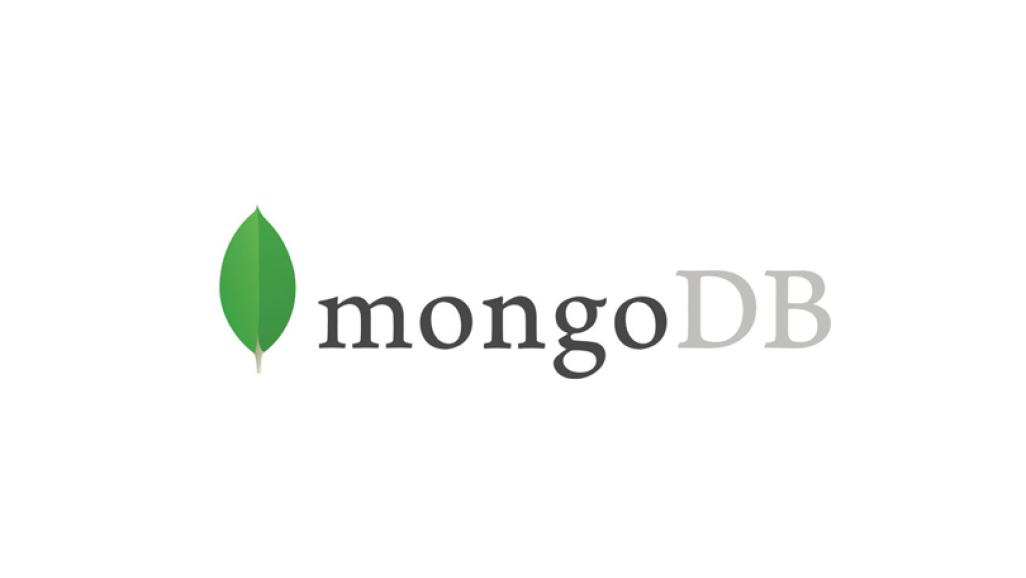
\includegraphics[width=8cm,height=3.3cm,keepaspectratio]{images/mongodb}
\end{center}
MongoDB is a cross-platform document-oriented database program. Classified as a NoSQL database program, MongoDB uses JSON-like documents with schema. Some of the main features of MongoDB are:

\begin{itemize}
    \item Ad-hoc queries (MongoDB supports field, range query, and regular-expression searches)
    \item Indexing (Fields in a MongoDB document can be indexed with primary and secondary indices)
    \item File storage (MongoDB can be used as a file system, called GridFS, with load balancing and data replication features over multiple machines for storing files)  
\end{itemize}

For this project, MongoDB was used as the main database. It stores user details and user sorts. To write to the database, a request is first made through the application. Using a proxy, these requests are delegated to a flask application. The flask application then processes the request and will then access the database to perform a certain action (such as writing user details to the database, accessing user details, storing user sorts, etc). 

\subsubsection{Advantages}
There are a number of advantages to using MongoDB:

\paragraph{Schema-less NoSQL Database}
MongoDB is a schema-less NoSQL database, meaning there is no need to design the schema of the database when using MongoDB. The code defines the schema.

\paragraph{Performance}
Performance of MongoDB is much higher than compared to any relational database.

\paragraph{Internal Memory}
MongoDB uses internal memory for storage which enables faster access to the data.

\paragraph{No Joins}
MongoDB doesn't use complex joins. There is no relationship among data in MongoDB.

\paragraph{JSON}
MongoDB supports JSON. Because MongoDB uses JSON format to store data, it is very easy to store arrays and objects.

\subsubsection{Disadvantages}
There are a few disadvantages to using MongoDB:

\paragraph{High Memory}
MongoDB uses high memory for data storage.

\paragraph{Document Size Limit}
MongoDB has a limit to the size of documents it can store.

\paragraph{Lack Of Transaction Support}
MongoDB does not support transactions.
\par
\medskip
\par
\medskip

\subsection{PythonAnywhere}
\par
\medskip
\begin{center}
    
\includegraphics[width=8cm,height=3.3cm,keepaspectratio]{images/pythonanywhere}
\end{center}
PythonAnywhere is an online integrated development environment (IDE) and web hosting service (Platform as a service) based on the Python programming language. it provides in-browser access to server-based Python and Bash command-line interfaces, along with a code editor with syntax highlighting. Program files can be transferred to and from the service using the user's browser. Web applications hosted by the service can be written using any WSGI-based application framework. For this project, the user authentication side of things was initially handled entirely by Firebase. However, as suggested by my supervisor, I decided to implement registering a user, logging a user into the application etc. myself. The functionality for this was written in Python and could be accessed by the application by using a proxy to delegate any requests made by the application to the Flask server. However, to enable the functionality to be accessed from anywhere (and, in turn, remove the need to run the Flask server alongside the application everytime), I decided to use PythonAnywhere. EXPLAIN

\subsubsection{Advantages}
There are a number of advantages to using PythonAnywhere:

\paragraph{Always running}
Even on a free tier account, PythonAnywhere never sleeps (compared to something like Heroku). This means real time services are viable with PythonAnywhere.

\paragraph{Fully configured}
PythonAnywhere gives you a fully configured Python environment...

\paragraph{Free}
PythonAnywhere is free to use. On a free tier account, web applications stay running 24/7 for 3 months. After 3 months, it will shut down. However, one needs only to start it up again.

\subsubsection{Disadvantages}

\paragraph{Python-only on the server side}
You are free to use JavaScript in your web pages and so on, but you can't use Rails or Node on the server side of things.

\paragraph{No WebSocket support}